\documentclass[11pt,a4paper]{article}
\usepackage[margin=25mm]{geometry}
\usepackage[T1]{fontenc}
\usepackage{mathpazo,microtype,amsmath,amssymb,amsthm,graphicx,booktabs,array,xcolor,enumitem}
\usepackage[numbers,sort&compress]{natbib}
\usepackage[colorlinks=true,linkcolor=black,citecolor=black,urlcolor=blue]{hyperref}
\usepackage{caption}
\captionsetup{font=small,labelfont=bf}
\makeatletter
\setlength{\@fptop}{0pt}
\setlength{\@fpsep}{18pt}
\setlength{\@fpbot}{0pt plus 1fil}
\makeatother
\setlength{\parindent}{1em}
\setlength{\parskip}{2pt}
\setlength{\emergencystretch}{3em}
\newtheorem{proposition}{Proposition}
\newtheorem{corollary}{Corollary}
\newcommand{\LCC}{\operatorname{LCC}}
\newcommand{\E}{\mathbb{E}}
\title{Preserving Recall Calibration through Connected-Component Filtering in Polyp Segmentation}
\author{Shivam Gupta\\\small Independent Researcher, India\\\small\href{mailto:shivam1720406@gmail.com}{shivam1720406@gmail.com}}
\date{14 October 2026}
\begin{document}
\maketitle
\begin{abstract}
Recall calibration for polyp segmentation can be invalidated by a subsequent mask-cleanup operation. We audit largest-connected-component (LCC) filtering, separating deletion of true-positive pixels at a fixed calibrated threshold from nonmonotonicity across thresholds. A running-union component-persistence completion is the smallest nested family containing the LCC outputs on a fixed grid; an established conformal loss-envelope baseline instead retains a single-component output. We evaluate fixed published PraNet and Polyp-PVT models on 701 distinct images from four public polyp datasets after removing 37 exact test repeats. In 500 shared calibration/evaluation splits, PraNet mean missed annotated area increased from 9.36\% to 48.64\% when LCC cleanup followed raw-mask calibration at a 10\% target. Persistence and loss-envelope calibration attained 8.99\% and 9.16\%, with mean output areas 39.43\% and 92.54\% of the frame. For Polyp-PVT, cleanup increased missed area from 9.75\% to 13.53\%; persistence calibration attained 9.78\%. A classical anchor-component control attained 9.01\% missed area with 28.01\% frame area for PraNet. The study releases code, complete threshold-path statistics, and sensitivity analyses. The results support calibrating the final returned mask and measuring cleanup-induced deletion; the guarantees concern expected image-level missed area under exchangeability, rather than clinical detection or resection outcomes.
\end{abstract}

\noindent\textbf{Keywords:} colonoscopy; polyp segmentation; conformal risk control; connected components; software validation.

\section{Introduction}
A calibrated segmentation pipeline makes a statement about its final output. In practice, the mask displayed to an endoscopist can differ from the threshold mask used during calibration. A common simplification retains only the largest connected component (LCC), an operation previously evaluated for polyp detection and segmentation~\cite{cleanup}. This removes isolated false predictions but can also delete annotated polyp pixels. We ask whether recall calibration survives this apparently routine change, how often the failure mechanism occurs in public benchmark predictions, and which corrections are useful when cleanup is retained.

The distinction has operational relevance. Endoscopy AI is an established product category: the FDA classified GI Genius as a gastrointestinal lesion detection system in 2021~\cite{fda}. We do not evaluate that device or assert that it uses LCC filtering. Instead, we study a reproducible component of a segmentation pipeline that could be tested during product validation. Our endpoint is the fraction of annotated polyp area omitted from a binary image mask. It is neither adenoma detection rate nor evidence of complete resection.

Two problems must be separated. First, deleting pixels \emph{after} calibrating a raw mask increases its missed-area loss even when the cleanup rule is fixed. Second, recalibrating an LCC-filtered family with the ordinary monotone conformal risk control (CRC) formula does not automatically repair the guarantee: when another component becomes larger, the selected component can switch and the loss can increase as the raw mask expands. This is a property of the output operation, independent of network retraining or probability calibration.

We contribute a paired audit of these two mechanisms on fixed PraNet and Polyp-PVT predictions, a transparent comparison of two corrections and standard connected-filter controls, and an executable artifact containing per-image paths, split assignments, duplicate exclusions, and mathematical checks. The corrections apply established calibration and morphology principles; the contribution is their controlled study at the final-mask stage of polyp segmentation. We use the descriptive name \emph{component-persistence completion} for the running union of selected components. We do not claim a new general conformal theorem.

\section{Related work and contribution boundary}
CRC controls the expectation of bounded monotone losses and already includes a polyp-segmentation application~\cite{crc}. Its Corollary~1 explicitly handles nonmonotone losses by replacing each loss with a suffix supremum. That construction is our loss-envelope comparator, not an original result. Recent work studies stability-based nonmonotone calibration~\cite{nonmono}, conditional risk adaptation~\cite{cra}, and training for conformal efficiency~\cite{crt}. None of these establishes that a raw-mask guarantee is invariant to an uncalibrated pixel-deletion step.

Morphological outer prediction sets and false-positive confidence masks have also been studied~\cite{morph,fp}. Connected operators, area filters, and component-tree representations are classical~\cite{connected}. We use fixed-marker reconstruction and area opening as established controls. Lu et al.~\cite{instance} construct confidence sets of alternative instance masks; their Appendix~H.1 already ensures nestedness after removing duplicate candidate masks in a CRC baseline. This is close conceptual precedent for preserving nestedness through postprocessing. Our setting differs in its output and loss: one binary polyp mask, LCC deletion of foreground pixels, and missed annotated area rather than the existence of a high-IoU alternative mask.

PraNet supplies a published segmentation model~\cite{pranet}. Yeh et al.~\cite{crt} supply a processed benchmark and its original pretrained checkpoint. Our study changes no model parameters and does not compete for state-of-the-art Dice. It evaluates the composition of prediction, cleanup, and calibration. The targeted literature search did not identify the same LCC recall-transfer audit, but it cannot establish absolute priority or exclude unpublished work.

\section{Final-mask recall and component persistence}
\subsection{Setup and estimand}
Let $\Omega$ be a finite rectangular pixel grid, $Y\subseteq\Omega$ a nonempty annotated foreground mask, and $s_x(p)\in[0,1]$ a fixed model score. Choose descending thresholds $t_0\ge\cdots\ge t_m=0$ independently of calibration labels and define
\begin{equation}
 C_j(x)=\{p:s_x(p)\ge t_j\},\qquad
 L(M,Y)=1-\frac{|M\cap Y|}{|Y|}.
 \label{eq:loss}
\end{equation}
The raw masks are nested, $C_j\subseteq C_{j+1}$, so their missed-area losses decrease. Each image contributes equally, regardless of its polyp area. Pixelwise pooled recall would define a different estimand. For empty annotation masks a separate background endpoint is required; the present public benchmark contains positive images only.

For a fixed mask family with decreasing losses $L_i(j)\in[0,1]$, standard CRC selects
\begin{equation}
 \widehat j=\min\left\{j:\frac{\sum_{i=1}^{n}L_i(j)+1}{n+1}\le\alpha\right\}.
 \label{eq:crc}
\end{equation}
Under exchangeability of the calibration images and a future image, with a fixed predictor and family, $\E L_{n+1}(\widehat j)\le\alpha$~\cite{crc}. The expectation includes calibration randomness. This is not a per-image recall guarantee, a confidence bound conditional on the realized calibration set, or a guarantee under source shift. The full-frame terminal mask has zero loss; all reported calibration sizes permit a passing terminal action.

\subsection{Deletion and switching are different mechanisms}
Write $D_j(x)=\LCC(C_j(x))$, with a fixed pixel adjacency and deterministic tie breaking. At any fixed threshold,
\begin{equation}
 L(D_j,Y)-L(C_j,Y)=\frac{|Y\cap(C_j\setminus D_j)|}{|Y|}\ge0.
 \label{eq:deletion}
\end{equation}
Thus a bound on raw-mask risk transfers to cleaned masks only with an additional bound on the deleted true-positive fraction. An empirical calibration of the raw mask alone supplies no such bound.

\begin{proposition}[Universal transfer and monotonicity]
For a deterministic postprocessor $T$, $L(T(S),Y)\le L(S,Y)$ for every nonempty $Y$ if and only if $S\subseteq T(S)$. Also, $L(T(A),Y)\ge L(T(B),Y)$ for every nonempty $Y$ whenever $A\subseteq B$ if and only if $T$ is increasing under set inclusion.
\end{proposition}
\begin{proof}
For the first claim, inclusion suffices. If $p\in S\setminus T(S)$, choose $Y=\{p\}$ to obtain losses zero and one. For the second, an increasing $T$ suffices. If $p\in T(A)\setminus T(B)$ for some $A\subseteq B$, the same singleton mask reverses the required loss inequality.
\end{proof}
These are universal statements over annotation sets, not claims that clinical annotations are single pixels. They identify which guarantees require recalibration or additional assumptions. A nontrivial anti-extensive filter cannot preserve every raw-mask recall bound automatically.

LCC is anti-extensive but not increasing. Consider two disconnected foreground regions: a two-pixel region $A$ with score $0.9$ and a three-pixel region $B$ with score $0.8$. With $Y=A$, lowering the threshold from $0.9$ to $0.8$ changes the LCC output from $A$ to $B$, and the loss rises from zero to one. At threshold zero the grid is connected and loss returns to zero. The nonmonotone path is verified in the released tests. This removes the usual monotone-CRC justification for naive LCC recalibration; it does not prove that every finite dataset will exhibit risk above its target.

\subsection{Two corrections and two classical controls}
\paragraph{Component-persistence completion.}
Define
\begin{equation}
 P_j(x)=\bigcup_{k=0}^{j}D_k(x).
 \label{eq:prefix}
\end{equation}
This is nested and satisfies $D_j\subseteq P_j\subseteq C_j$. It retains every pixel previously displayed as part of a winning component. It may contain several disconnected components. We apply Eq.~\eqref{eq:crc} to $L(P_j,Y)$ using the same path at calibration and evaluation.

\begin{proposition}[Minimal nested completion]
Among all nested families $H_j$ satisfying $D_j\subseteq H_j$ at every grid index, $P_j$ is the pointwise smallest: $P_j\subseteq H_j$. Moreover, $P_j$ is the union of the selected raw components over the threshold prefix and is contained in the current raw mask.
\end{proposition}
\begin{proof}
For $k\le j$, nesting implies $D_k\subseteq H_k\subseteq H_j$. Taking the union gives $P_j\subseteq H_j$. Since $D_k\subseteq C_k\subseteq C_j$, the union is contained in $C_j$.
\end{proof}
This minimality concerns set inclusion for a fixed threshold grid. It does not imply optimal expected area among all possible calibrated segmenters, or minimal area after different thresholds have been selected.

\paragraph{Established loss-envelope calibration.}
Keep the LCC output but calibrate the decreasing upper loss
\begin{equation}
 U_i(j)=\max_{k\ge j}L(D_k(X_i),Y_i).
 \label{eq:envelope}
\end{equation}
This is exactly the finite-grid version of CRC Corollary~1~\cite{crc}. Because $L(D_j,Y)\le U(j)$, applying Eq.~\eqref{eq:crc} to $U$ controls expected final LCC loss under the same exchangeability assumptions. It preserves a single-component output at the cost of potentially relaxing the threshold. No labels are required to form evaluation outputs once the common threshold is calibrated.

\paragraph{Increasing connected filters.}
The anchor control retains the component containing a fixed maximum-score pixel, using the first raster position to break ties. The anchor is chosen from the score image once and does not change with the threshold. Components containing that marker can only grow or merge. The area-opening control retains every component with at least 64 pixels at each threshold. Any retained component remains inside a component at least as large at a later threshold. Both families are nested and admit standard CRC after calibration. Their morphology is established~\cite{connected}; neither universally preserves the risk of an already calibrated raw mask.

\paragraph{Implementation.}
The reference implementation labels all threshold masks directly, uses eight-connectivity, and accumulates a Boolean running union. For $G$ thresholds and $V$ pixels, this costs $O(GV)$ work per image and $O(V)$ mask memory when streamed, in addition to recorded statistics. An already selected operating threshold requires only its prefix for persistence. The envelope requires all calibration thresholds, but deployment evaluates one threshold and one LCC operation. Component-tree implementations~\cite{connected} could reduce repeated work; real-time hardware performance is not established here.

\section{Experimental design}
\subsection{Data, provenance, and independence}
We use the processed test release from Yeh et al.~\cite{crt}, which contains Kvasir-SEG~\cite{kvasir}, CVC-ClinicDB~\cite{clinic}, CVC-ColonDB~\cite{colondb}, and ETIS-LaribPolypDB~\cite{etis}. The preparation notebook corrects mask-format issues and omits CVC-300 because it overlaps CVC-ColonDB. We retain the release's original train/test allocation. Before inference we hash decoded RGB pixels with their dimensions, discard any test image matching a training image, and retain only the first test instance of each hash in lexicographic path order. Identical images with different masks are therefore not counted as independent test units. Excluded filenames and reasons are released.
\begin{table}[htbp]
\centering\small
\caption{Released test images and retained distinct images. Path diagnostics use the primary eight-connected, transformed 257-point threshold grid.}
\label{tab:data}
\begin{tabular}{lrrrr}\toprule
Source & Released & Retained & Nonnested LCC & Loss increase\\\midrule
CVC-ClinicDB & 62 & 62 & 54 & 53 \\
CVC-ColonDB & 380 & 346 & 267 & 239 \\
ETIS-LaribPolypDB & 196 & 193 & 153 & 129 \\
Kvasir-SEG & 100 & 100 & 80 & 76 \\
\midrule Total & 738 & 701 & 554 & 497 \\
\bottomrule\end{tabular}\end{table}
Patient and sequence identifiers are unavailable in the evaluated release. Exact duplicate removal cannot establish patient separation, remove near-duplicate frames, or establish independence across sources. We interpret random splitting as an experiment on the finite image pool. The mathematical exchangeability result is stated separately from claims about future clinical populations.

\subsection{Model and processing}
We use the published PraNet-19 checkpoint without fitting or selection. A secondary architecture replication uses the released Polyp-PVT checkpoint~\cite{pvt}, with the sum of its two output logits as in the official testing implementation. Its redundant standalone-backbone initialization is removed before the complete checkpoint is strictly loaded; no learned parameter is changed. Input RGB images are resized to $352\times352$ using Pillow bilinear interpolation, mapped to $[0,1]$, and normalized with ImageNet mean and standard deviation. PraNet runs in evaluation mode with frozen running statistics. The final output is passed through the sigmoid directly, without per-image min--max normalization or fitted temperature. For Polyp-PVT, adaptive average pooling uses CPU evaluation because the MPS backend does not support its non-divisible pooling shapes; all remaining forward operations use MPS. Binary annotations are resized to the same grid by nearest neighbor. The evaluated endpoint is explicitly the resized annotation, rather than a native-resolution boundary metric. All source and weight hashes are recorded. Apple MPS inference is compared with CPU inference for the first three images.

\subsection{Paired comparisons and statistics}
An initial 257-point uniform probability grid caused the primary target to select a full-frame mask for every split. We preserve this pilot and amended the grid to resolve saturated scores: $t(u)=\operatorname{sigmoid}(10\operatorname{logit}(u))$, for 257 equally spaced $u$ values from one to zero, with exact endpoints. This is a fixed spacing rule, motivated by the temperature-10 scoring in the original CRC code, rather than temperature fitting. Rounding of the stored float32 sigmoid scores can affect extreme thresholds; no calibrated claim is attached to the score values themselves. Eight-neighbor adjacency and first-raster-label tie breaking are fixed. The initial exploratory protocol preceded prediction analysis; the documented grid amendment and addition of the transformer replication followed the degenerate pilot. Neither is described as preregistered. At $\alpha=0.10$, we compare raw CRC; raw CRC followed by LCC; naive LCC recalibration; CRC on the persistence completion; the established LCC loss envelope; anchor CRC; and area-opening CRC. Sensitivity targets are $0.05$ and $0.20$. The same 500 random unstratified half-pool splits (NumPy generator seed 20406) are used for every method and target. Calibration uses the smaller half and evaluation the larger half. Split assignments can be reconstructed exactly from the seed and released manifest.

We report mean evaluation missed area, predicted area divided by frame area, Dice, and selected threshold. The spread across repeated splits describes partition sensitivity; it is not a confidence interval from 500 independent studies. The raw-versus-cleaned comparison uses paired outputs at the same calibrated threshold. We also count images whose LCC path is not nested and those whose annotated-area loss increases at any adjacent grid step. A supplementary descriptive analysis chooses a raw CRC threshold using the whole pool and bootstraps the per-image cleanup penalty (5,000 image resamples, seed 809). Its interval assumes image sampling and does not correct frame correlation; it is not held-out performance. Source-held-out analysis calibrates on the other three sources and evaluates the remaining source as a distribution-shift stress test.

\section{Results}
The primary transformed grid revealed nonnested LCC paths in 554/701 images (79.0\%) and adjacent increases in annotated-area loss in 497/701 (70.9\%; Table~\ref{tab:data}). The two quantities differ because deleted pixels need not intersect the reference annotation. Figure~\ref{fig:mechanism} isolates the mechanism in an exact synthetic example.

\begin{figure}[htbp]\centering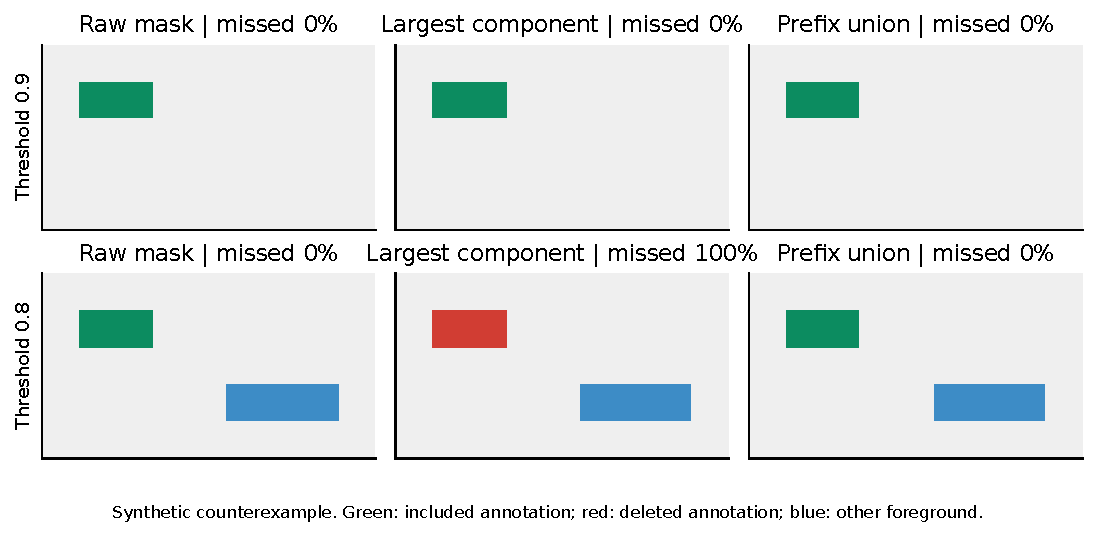
\includegraphics[width=.94\linewidth]{../figures/mechanism.pdf}\caption{A synthetic switch between two disconnected regions. Lowering the threshold adds pixels to the raw mask but replaces its largest component. The two-pixel reference annotation is then lost. The running union retains it. Colors distinguish annotated foreground from other selected pixels.}\label{fig:mechanism}\end{figure}

\subsection{Cleanup after raw calibration}
Across the shared splits, raw CRC attained mean missed area 9.36\%, whereas subsequent LCC cleanup increased it to 48.64\% (Table~\ref{tab:primary}). The paired increase was 39.29 percentage points. Cleanup removed more than 1\% of annotated area in a mean 45.42\% of evaluation images. The predicted frame area changed from 33.17\% to 23.89\%, a decrease in displayed area accompanied by a substantial recall cost. These are properties of the sampled images, not estimates of clinical polyp miss rate.

At the descriptive full-pool calibrated threshold $t=5.7e-05$, the mean per-image cleanup penalty was 41.82 percentage points (image-bootstrap 95\% interval 38.31--45.39). In 336 images the penalty exceeded one percentage point. This threshold uses the entire pool and is not a held-out operating-point estimate.

\begin{table}[htbp]\centering\small
\caption{PraNet primary evaluation at target 10\% missed annotated area. Values average 500 shared splits, with 350 calibration and 351 evaluation images. The range is the 2.5th--97.5th percentile of split risks, not a population confidence interval. All numerical columns except Dice are percentages.}
\label{tab:primary}
\begin{tabular}{lrrrr}\toprule
Procedure & Missed area & Split range & Frame area & Dice\\\midrule
Raw CRC & 9.36 & 6.39--13.51 & 33.17 & 0.345 \\
Raw CRC + LCC & 48.64 & 29.39--62.81 & 23.89 & 0.321 \\
LCC recalibration & 9.16 & 5.56--14.13 & 92.54 & 0.135 \\
Prefix union CRC & 8.99 & 5.42--12.69 & 39.43 & 0.300 \\
LCC envelope CRC & 9.16 & 5.56--14.13 & 92.54 & 0.135 \\
Anchor CRC & 9.01 & 5.10--12.47 & 28.01 & 0.579 \\
Area opening CRC & 9.35 & 6.41--13.57 & 33.35 & 0.343 \\
\bottomrule\end{tabular}\end{table}
\begin{figure}[htbp]\centering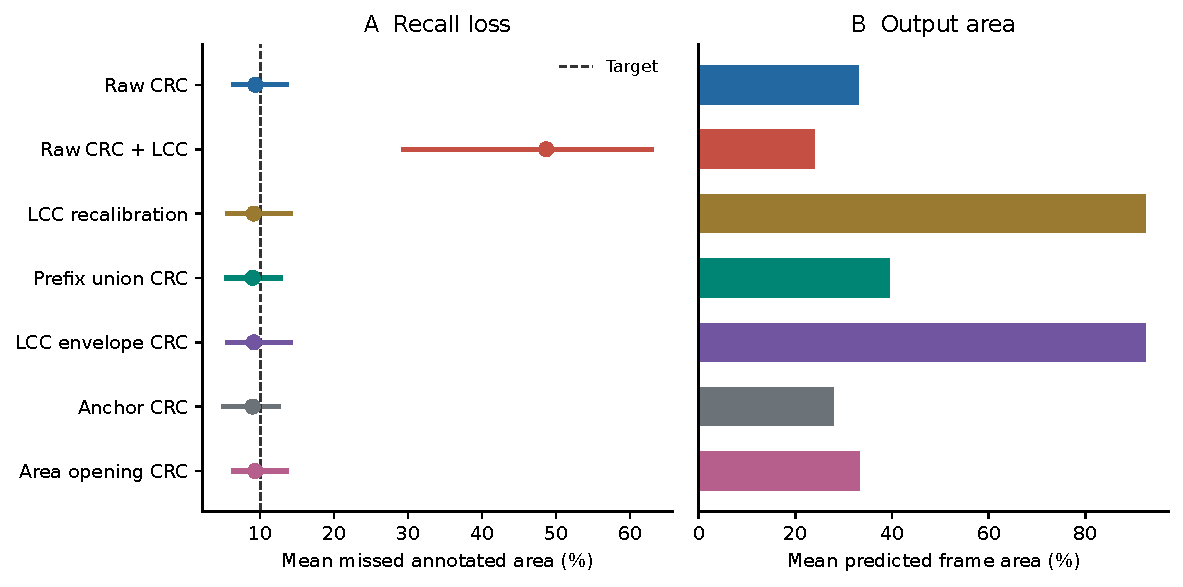
\includegraphics[width=\linewidth]{../figures/primary.pdf}\caption{PraNet evaluation at a 10\% target. Points are split-mean risks; horizontal lines show the central 95\% of risks across overlapping random splits. Bars report mean predicted frame area. The dashed line marks the target.}\label{fig:primary}\end{figure}

\subsection{Recalibration and output constraints}
Persistence CRC attained mean missed area 8.99\% with 39.43\% frame area. The established loss-envelope method attained 9.16\% with 92.54\% frame area while returning an LCC mask. Naive LCC recalibration attained 9.16\%; its empirical performance does not supply a general guarantee for nonmonotone paths. The anchor and area-opening controls attained 9.01\% and 9.35\%, respectively. Figure~\ref{fig:examples} shows two deliberately selected high-penalty cases, chosen by the largest cleanup penalty in distinct source datasets after excluding Kvasir images to avoid acquisition text in the display, rather than representative random images.

\begin{figure}[htbp]\centering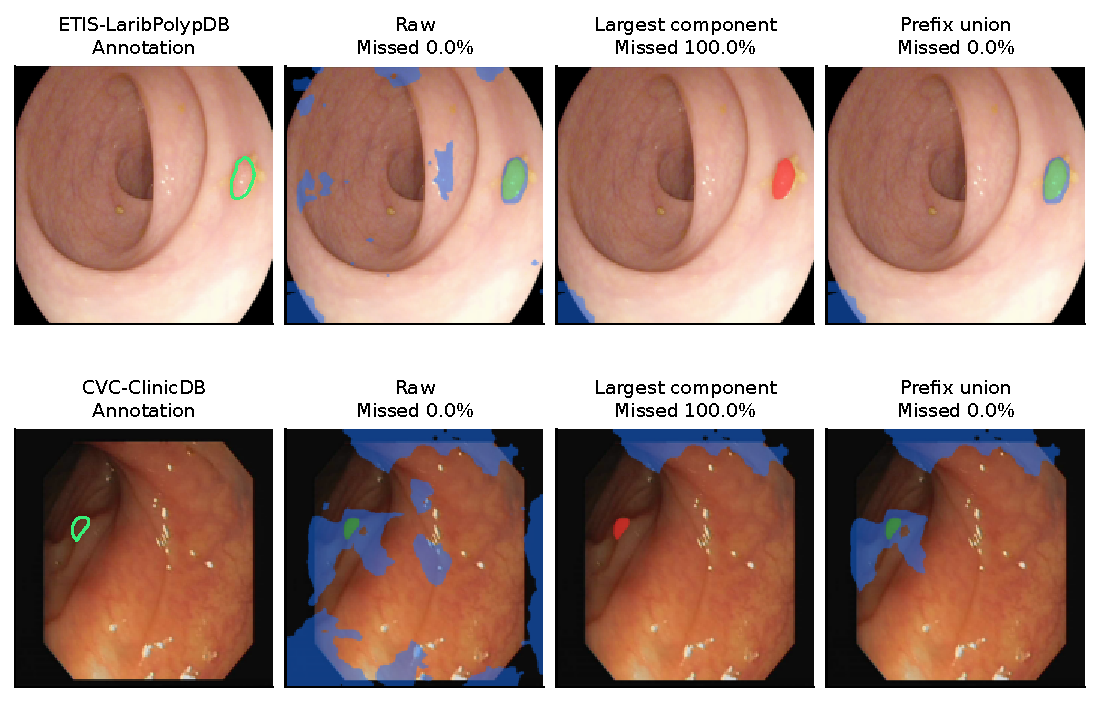
\includegraphics[width=\linewidth]{../figures/examples.pdf}\caption{Two high-penalty PraNet examples at the same descriptive full-pool threshold. Green denotes included annotated area, red missed annotated area, and blue selected background. The prefix union is evaluated at this same threshold for mechanism illustration; its independently calibrated operating point differs. These examples are selected by outcome and do not estimate effect frequency.}\label{fig:examples}\end{figure}

\subsection{Transformer replication and sensitivity analyses}
On Polyp-PVT, the same intervention changed mean missed area from 9.75\% to 13.53\%. Persistence, envelope, and anchor calibration attained 9.78\%, 8.97\%, and 9.82\%, respectively. The transformer had 469/701 nonnested LCC paths and 449/701 paths with an annotated-loss increase. The model comparison changes the magnitude of the effect; neither model is selected on these results.

\begin{table}[htbp]\centering\small
\caption{Polyp-PVT replication at the 10\% target, with the same images and 500 paired splits. All numerical columns except Dice are percentages; split ranges are partition sensitivity.}
\label{tab:pvt}\begin{tabular}{lrrrr}\toprule
Procedure & Missed area & Split range & Frame area & Dice\\\midrule
Raw CRC & 9.75 & 7.31--12.67 & 8.91 & 0.822 \\
Raw CRC + LCC & 13.53 & 10.89--16.33 & 8.59 & 0.818 \\
LCC recalibration & 10.11 & 7.44--13.55 & 18.33 & 0.729 \\
Prefix union CRC & 9.78 & 6.76--12.90 & 10.06 & 0.807 \\
LCC envelope CRC & 8.97 & 4.97--12.44 & 98.48 & 0.131 \\
Anchor CRC & 9.82 & 6.89--13.55 & 11.51 & 0.785 \\
Area opening CRC & 9.75 & 7.27--12.69 & 8.90 & 0.822 \\
\bottomrule\end{tabular}\end{table}

At the primary target, naive LCC recalibration and envelope calibration selected the same grid index in 500/500 PraNet splits. At the primary target, naive LCC recalibration and envelope calibration selected the same grid index in 32/500 Polyp-PVT splits. Naive recalibration had mean Polyp-PVT risk 10.11\%, slightly above the 10\% target; the split variability and finite Monte Carlo experiment do not establish a systematic target violation. Consequently, the experiment demonstrates failure of transferring raw-mask calibration through cleanup, but does not establish that naive final-mask recalibration fails empirically at this target.

For PraNet with four-connectivity, raw/cleaned mean missed areas were 9.36\%/48.64\%; persistence/envelope/anchor risks were 8.99\%/9.18\%/9.01\%. For PraNet with 513-point grid, raw/cleaned mean missed areas were 9.64\%/45.93\%; persistence/envelope/anchor risks were 9.49\%/9.50\%/9.47\%. The target sensitivity results and source-held-out stress results are included in Appendix~\ref{app:additional}.

The classical anchor control used less mean frame area than persistence in the primary PraNet comparison (28.01\% versus 39.43\%) and attained a higher mean Dice (0.579 versus 0.300). Thus the running-union construction is useful for preserving a display-history constraint, but the data do not support preferring it over established increasing filters solely for segmentation utility.



\section{Discussion}
\subsection{What the audit changes in practice}
The evaluated risk attaches to the mask family and calibration rule together. A software service that changes its component filtering after calibrating a raw mask changes the endpoint for which the guarantee was established. Equation~\eqref{eq:deletion} provides an exact audit quantity for this change. The recommended integration check is therefore specific: version the score preprocessing, threshold grid, connectivity, tie rule, and postprocessor alongside the calibration artifact, and evaluate the output actually returned by the service.

The two corrections answer different product constraints. Persistence permits additional regions and prevents the disappearance of earlier winning pixels, with a minimality statement on the fixed grid. The established envelope retains one component and calibrates against future reversals of its loss path. The anchor and area-opening controls test whether ordinary increasing morphology is sufficient without carrying component history. Method selection should consider area, false positives, connectedness, and compute, rather than recall alone. Enlarging a mask can reduce missed area while worsening delineation utility. A full-frame mask always has zero missed-area loss and can be clinically unhelpful.

\subsection{Commercial translation}
The immediate application is a model-agnostic validation module for endoscopy segmentation vendors or research inference services: compare the calibrated intermediate output with the displayed final mask, quantify deleted annotated area, and rerun calibration when the pipeline changes. This is a technical product hypothesis supported by the existence of endoscopy AI systems~\cite{fda}, not a market-demand estimate. The study does not evaluate clinician workload, prospective detection, resection safety, revenue, or willingness to pay. A commercial implementation would need appropriate rights to model weights and data; the research-use conditions of PraNet and Kvasir-SEG do not become commercial permissions through this study. The released original audit code is separate from those upstream assets. We make no patentability claim for these elementary constructions.

\subsection{Limitations and validation priorities}
The experiment uses two published architectures with one checkpoint each. Repeated partitions are calibration-split sensitivity, not model-seed replication. Conclusions about the frequency or magnitude of cleanup effects may change with stronger modern segmenters. The exact set-theoretic mechanism, however, does not depend on architecture. The exploratory design does not constitute preregistration, and benchmarking several corrections does not establish that the best observed result will generalize to a new site.

All images contain annotated foreground. We cannot evaluate false alarms on normal mucosa, patient-level detection, clinical lesion counts, or video persistence. The mask labels are reference annotations rather than error-free biological truth. Resizing can change small structures, and the finite threshold grid can miss component switches between grid points. Four-connectivity and a denser grid for PraNet examine selected implementation sensitivities but do not remove those limitations. Patient identifiers, prospective source-specific calibration, multiple contemporary segmenters, negative frames, and native-resolution assessment are priorities before deployment.

\section{Conclusion}
Largest-component filtering can delete true-positive polyp pixels from a recall-calibrated mask and can make an otherwise nested threshold path nonmonotone. These are distinct, testable pipeline properties. Calibration of the final procedure, with established loss envelopes or a nested mask construction, provides an explicit route to recover the standard expected-loss justification. The public benchmark quantifies the associated recall and area trade-offs; it does not establish a clinical safety or detection benefit.

\paragraph{Data and code availability.}
Original analysis code, experimental protocol, per-image sufficient statistics, reproducibility instructions, and manuscript source are available at \url{https://github.com/shi1720/polyp-component-persistence}. Images and weights are obtained from their original releases and are not redistributed. The artifact records checksums and the upstream revision.
\paragraph{Funding and competing interests.}
No external funding was received for this study. The author founded Siloed, an AI consultancy. No Siloed product is evaluated in this study.

\bibliographystyle{plainnat}
\bibliography{references}

\appendix
\section{Finite-grid guarantee and implementation checks}
For completeness, the finite-grid CRC argument can be stated without a continuity assumption. On $n+1$ exchangeable images define the symmetric full-data index $j^*$ as the first index with mean loss at most $\alpha$. For each omitted image $i$, the index $\widehat j_{-i}$ selected using Eq.~\eqref{eq:crc} is feasible for the full-data condition because the omitted loss is at most one. Hence $\widehat j_{-i}\ge j^*$. For decreasing losses,
\[
 \frac{1}{n+1}\sum_{i=1}^{n+1}L_i(\widehat j_{-i})
 \le\frac{1}{n+1}\sum_{i=1}^{n+1}L_i(j^*)\le\alpha.
\]
Exchangeability gives the expected-loss bound for a future image. For the envelope procedure apply this argument to $U_i$ and then use $L(D_j,Y)\le U_i(j)$. This is a finite-grid specialization of established CRC~\cite{crc}. It does not justify naive LCC recalibration, whose loss need not decrease.

The released test suite enumerates all $3^6=729$ score images on a $2\times3$ grid for both four- and eight-connectivity. It verifies nesting and containment for raw, persistence, anchor, and area-opening families and verifies the running-union definition exactly. A separate two-region example verifies loss sequence $(1,0,1,0)$ for LCC. Suffix-envelope values are compared with direct suffix maxima. Finally, an exact leave-one-out check tests the CRC inequality on 100 finite populations at three targets. These checks test the implementation and mathematical invariants; benchmark evidence comes from the public images.

\section{Reproducibility details}
The reference environment uses Python 3.12, PyTorch 2.14.1, NumPy 2.5.4, SciPy 1.18.1, Pillow 12.3.0, and timm 1.0.30 on macOS/Apple Silicon. A complete dependency lock file is released. CPU computations use two PyTorch threads; path generation uses two workers. Model inference runs once per retained image. Subsequent splits reuse the same fixed paths and do not refit a model or postprocessor.

The maximum absolute CPU--MPS sigmoid differences over the first three images were 2.4e-05 for PraNet and 2.84e-05 for Polyp-PVT. Reported inference times, including reference checks but excluding data download and duplicate hashing, were 220.8 and 161.6 seconds, respectively. These are reference-run timings, not deployment latency benchmarks.

\begin{table}[htbp]\centering\small
\caption{Reference artifact identifiers. Complete hashes and download URLs are in the machine-readable asset manifest.}
\begin{tabular}{ll}\toprule
Asset & SHA-256 prefix / Git revision prefix\\\midrule
Processed data archive & \texttt{554b9f23ba697083}\\
PraNet checkpoint & \texttt{1e178247113e4b87}\\
Polyp-PVT checkpoint & \texttt{aef5ac34f7795b85}\\
Data/architecture source revision & \texttt{b9b2276e3e1ccf26}\\
Polyp-PVT source revision & \texttt{cd71fbf9fcd8c32c}\\\bottomrule
\end{tabular}\end{table}

The artifact separates original code from third-party assets. The download script verifies data and checkpoint hashes, obtains pinned architecture files, and documents the initialization-only patch for Polyp-PVT. A released image manifest fixes ordering and duplicate retention. For each image, method, and grid point, the path files store missed fraction, frame-area fraction, and Dice. These sufficient statistics reproduce every split-level comparison without re-running a neural network. Figure regeneration additionally requires the upstream images and the inference cache. The uniform-probability-grid pilot remains available, including its full-frame outcome, to document the exploratory amendment.

\section{Additional benchmark results}\label{app:additional}
\begin{table}[htbp]\centering\small
\caption{Mean missed annotated area (\%) across shared splits at three targets. P denotes PraNet and V denotes Polyp-PVT. No entry is a per-patient result.}
\begin{tabular}{lrrrrrr}\toprule
 & P: 5\% & P: 10\% & P: 20\% & V: 5\% & V: 10\% & V: 20\%\\\midrule
Raw CRC & 4.29 & 9.36 & 19.79 & 4.70 & 9.75 & 19.75 \\
Raw CRC + LCC & 63.56 & 48.64 & 22.00 & 9.72 & 13.53 & 21.52 \\
LCC recalibration & 4.47 & 9.16 & 21.10 & 4.12 & 10.11 & 19.81 \\
Prefix union CRC & 4.33 & 8.99 & 19.82 & 4.70 & 9.78 & 19.79 \\
LCC envelope CRC & 4.47 & 9.16 & 19.25 & 4.12 & 8.97 & 18.63 \\
Anchor CRC & 4.44 & 9.01 & 19.82 & 4.71 & 9.82 & 19.89 \\
Area opening CRC & 4.29 & 9.35 & 19.79 & 4.70 & 9.75 & 19.75 \\
\bottomrule\end{tabular}\end{table}
\begin{table}[htbp]\centering\small\caption{PraNet source-held-out stress: missed annotated area (\%) when calibrating at 10\% on the other sources. Source shift is outside the exchangeability guarantee.}
\begin{tabular}{lrrrr}\toprule
Procedure & ClinicDB & ColonDB & ETIS & Kvasir\\\midrule
Raw CRC & 0.75 & 15.79 & 12.38 & 1.54 \\
Raw CRC + LCC & 68.05 & 23.19 & 54.12 & 57.90 \\
LCC recalibration & 12.63 & 15.13 & 3.37 & 8.15 \\
Prefix union CRC & 2.18 & 12.72 & 13.90 & 2.38 \\
LCC envelope CRC & 12.63 & 15.13 & 3.37 & 8.15 \\
Anchor CRC & 4.69 & 11.17 & 11.99 & 5.91 \\
Area opening CRC & 0.75 & 15.81 & 12.46 & 1.54 \\
\bottomrule\end{tabular}\end{table}
\begin{table}[htbp]\centering\small\caption{Polyp-PVT source-held-out stress: missed annotated area (\%) when calibrating at 10\% on the other sources. Source shift is outside the exchangeability guarantee.}
\begin{tabular}{lrrrr}\toprule
Procedure & ClinicDB & ColonDB & ETIS & Kvasir\\\midrule
Raw CRC & 2.58 & 17.17 & 7.68 & 5.17 \\
Raw CRC + LCC & 4.72 & 18.35 & 15.43 & 8.22 \\
LCC recalibration & 5.10 & 8.26 & 13.21 & 8.28 \\
Prefix union CRC & 4.08 & 12.99 & 11.25 & 6.99 \\
LCC envelope CRC & 9.80 & 12.60 & 9.39 & 2.12 \\
Anchor CRC & 7.22 & 11.79 & 10.16 & 8.47 \\
Area opening CRC & 2.58 & 17.13 & 7.68 & 5.18 \\
\bottomrule\end{tabular}\end{table}
Source-dependent risks can exceed the nominal target even for mathematically valid procedures when calibration and evaluation distributions differ. These stress results do not extend the finite-pool guarantee to clinical populations.

\end{document}
